\documentclass[10pt]{article}
\usepackage[left=1.0in,right=1.0in,top=1.0in,bottom=1.0in]{geometry}

% mostly stolen from 
% http://tex.stackexchange.com/questions/63357/automatically-generated-bingo-cards
%
% with a few additions myself
% Jesse Hamner, 2016

\usepackage{xstring}
\usepackage{pgffor}
\usepackage{tikz}
\usetikzlibrary{calc}
\usepackage{xparse}

\input{random.tex}
\newcount\randomnum
\ExplSyntaxOn

\seq_new:N \g_my_items_seq
\seq_new:N \l_my_tmp_items_seq
\seq_new:N \g_my_randomized_seq
\int_new:N \l_tmp_int
\msg_new:nnnn {bingo} {Too~few~items!} {Provide~at~least~24~items!}{}

\cs_generate_variant:Nn \seq_item:Nn {Nx}
\cs_generate_variant:Nn \seq_remove_all:Nn {Nx}

\NewDocumentCommand {\myItems} {m}
    {
      \seq_clear:N \g_my_items_seq % clear item list 
      \seq_gset_split:Nnn \g_my_items_seq {;} {#1} % put item list in seq
      \int_compare:nNnT {\seq_count:N \g_my_items_seq} < {24} {\msg_error:nn {bingo} {Too~few~items!}} % check whether there are enough items
    }

\NewDocumentCommand{\setItems}{}
{
\seq_set_eq:NN \l_my_tmp_items_seq \g_my_items_seq % put in temp seq so that multiple cards can be produced
\prg_replicate:nn {24} %generate random list of 24 items
    {
        \int_set:Nn \l_tmp_int {\seq_count:N \l_my_tmp_items_seq}% set current length of list
        \setrannum{\randomnum}{1}{\int_use:N \l_tmp_int} % choose random num up to length of seq
        \seq_put_right:Nx \g_my_randomized_seq {\seq_item:Nn \l_my_tmp_items_seq {\the\randomnum}}% grab corresponding item and put in tmp seq
        \seq_remove_all:Nx \l_my_tmp_items_seq {\seq_item:Nn \l_my_tmp_items_seq {\the\randomnum}}%delete that item from temp seq
    }
\seq_clear:N \l_my_tmp_items_seq %clear temp seq when done
}

\NewDocumentCommand {\NodeText}{}
    {
        \seq_gpop_right:NN \g_my_randomized_seq \l_tmpa_tl %pop item from randomized seq into token list
        \tl_use:N \l_tmpa_tl %use that item.
    }


\ExplSyntaxOff

\def\NumOfColumns{5}%
\def\Sequence{1, 2, 3, 4, 5}%
\newcommand{\sep}{1mm}

% make a nice identifier for the card (in case, say, there is more than one
% presidential debate, etc.)
\newcommand{\biglabel}{\vspace{0.2in}\begin{center}
\begin{LARGE}
Rawlins Hall Bingo

First Presidential Debate

25 September 2016

\end{LARGE}
\end{center}
}

% Although it doesn't save any code by breaking this out into its own 
% function (subroutine), it makes the code easier to parse down below
% in the for loop:
\newcommand{\drawthecard}{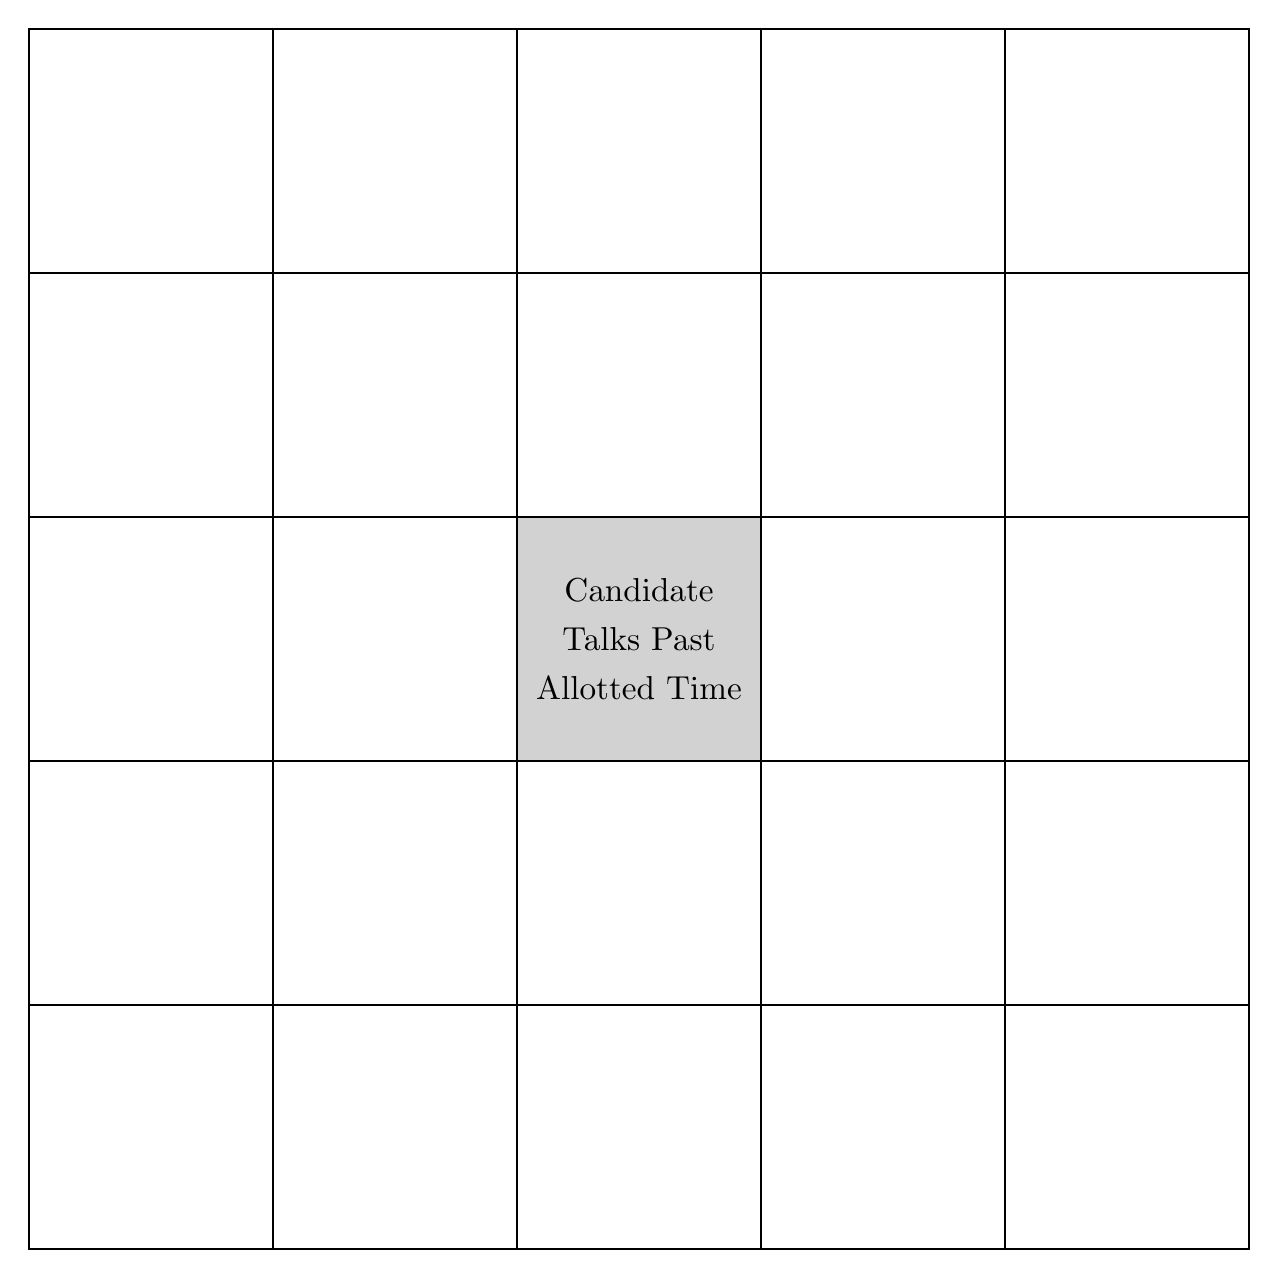
\begin{tikzpicture}[draw=black, thick, x=\Size,y=\Size]
\foreach \row in \Sequence{%
    \foreach \col in \Sequence {%
        \pgfmathtruncatemacro{\value}{\col+\NumOfColumns*(\row-1)}
        \pgfmathsetmacro{\ColRowProduce}{\col*\row}
        \IfEq{\ColRowProduce}{9}{% If is center square:
            \filldraw[fill=gray!35, draw=black] ($(\col,-\row)-(1,1)$) rectangle ($(\col,-\row)$) ;
% "Free Space" -- that's the joke:
           \node [scale=1.2] at ($(\col,-\row)-(0.5,0.3)$) {Candidate};
             \node [scale=1.2] at ($(\col,-\row)-(0.5,0.5)$) {Talks Past};
            \node [scale=1.2] at ($(\col,-\row)-(0.5,0.7)$) {Allotted Time};        }{
            \node [Square] at ($(\col,-\row)-(0.5,0.5)$) {\large \NodeText};
        }
    }
}    
\end{tikzpicture}
}

\newcommand{\Size}{3.1cm}
\newcommand{\Sizeinner}{3.0cm}
\tikzset{Square/.style={
inner sep=0pt,
text width=\Sizeinner, 
minimum size=\Size,
draw=black,
align=center,
}
}

\begin{document}
\pagestyle{empty}
%\myItems{this;will;produce;an;error;because;there;aren't;enough;items}

% These items are all contained in a separate file, deliberately broken out
% so that it's easier to read and parse without messing with the original
% LaTeX file:

%\myItems{``Believe me"; Tax returns; Benghazi; Shot of Bill Clinton in audience; Clinton Foundation; ``Make America Great Again"; Tim Kaine; Build ``the wall"; Heckler interrupts debate; Candidate talks past allotted time; Gun ban; NAFTA; Black Lives Matter; ``Basket of deplorables"; Alt-right; Florida; Mike Pence; Moderator interrupts candidate; Free market; ``My record shows ...''; Terrorism; Candidate demands an apology; John McCain; Pam Bondi; Health of candidate; Trump charity; ``Liberal media"; Shot of Melania Trump in audience; ``What do you have to lose?"; China; Taxes; Climate change; Middle East; Emails; ``I've employed thousands of people"; Joke about Trump's hair; Candidate says the other is ``disqualified"; Clinton mentions children--any children; Emails; Temperament; Transparency; ``Stronger Together"; NAFTA; Bankruptcy; Birther; Audience laughs; NATO; ``Tremendous success"; ``I can fix it"; President Obama; Ronald Reagan; Audience claps; Rigged; Trump says he was against the Iraq War; The Second Amendment; Trade agreement; Skittles; Income inequality; Top 1\%; Political correctness }

% read in the list of 'squares'
\myItems{``Believe me";
Make America Great Again;
Build a/the wall;
Liberal media;
``Tremendous";
We don't \emph{win} anymore;
International respect;
Small Town;
China;
Syria;
Israel;
Iran;
Mexico;
Russia;
North Korea;
Heckler interrupts speech;
The Middle Class;
Bernie Sanders;
Elizabeth Warren;
Mike Pence;
Alliances;
National Debt;
Trade Deals;
Infrastructure;
Clean Energy;
Coal;
Law and Order;
Terrorism;
Bipartisan;
Free market;
Free enterprise;
Freedom;
Taxes;
NAFTA;
US budget deficit;
Social Security;
Veterans;
The Second Amendment;
Transparency;
NATO;
``Leadership";
``I love \_\_\_\_\_.'';
the Supreme Court;
Immigration reform;
Obamacare;
Muslim ban;
Voter ID laws;
Voter fraud;
Russian ``Hacking";
``Wall Street";
``Main Street";
Russia;
Vladimir Putin;
Medicare;
ISIS;
Congress;
Refugees;
Impeachment;
Britain;
Names a small town;
Trade war;
Touts record Dow Jones;
Strongest military;
Farmers;
``Blue states";
Misprounounces word;
Points to guest;
``Nancy Pelosi";
Mar-a-lago;
Whistleblower;
``Disaster";
``Many people are saying";
Camera shows other Trumps;
Anyone sleeping;
Entitlement cuts;
``God bless America";
Mike Pompeo;
Ukraine;
NASA;
``Entrepreneurs"
}
% Trump says he was against the Iraq War;
%Twitter/Tweet;
%Trump apology;
%Glass Ceiling;
% America is already great;
% GOP withdrawing support for Trump;
% Sexual assault;
% Wikileaks;
% War on Women;
% Kellyanne Conway;
% Rape/Rapist;
% Citizens United;
% Moderator drops the hammer;
% Women's Rights;
% Amnesty;
% Islamophobia;
% What do you have to lose?;
% I've employed thousands of people;
% I can fix it;
% Political correctness;
% Crooked Hillary;
% Low energy;
% Rigged;
% Benghazi;
% Florida;
% Moderator becomes visibly frustrated;
% Candidate demands an apology;
% Unqualified;
%Clinton mentions children--\emph{any} children;
%Candidate mentions an endorsement;
%My record shows ...;
%On my first day in office;
%In my first hundred days;
% Clinton says using server was a mistake;
% Stronger Together;
% Deplorables;
% John McCain;
% Tim Kaine;
% Pam Bondi;
% President Obama;
% Bill Clinton;
% Ronald Reagan;
% Paid family leave;
% Missile Defense;
%America's place in the world;
% Single-payer Healthcare;
% More of the Same;
% Privatize Social Security;
% Community Policing;
% Stop and Frisk;
% Implicit Bias;
% Institutional Racism;
% Open Borders;
% LGBTQ rights;
% I have a plan;
% Bankruptcy;
% Tax returns;
% TPP;
% Income inequality;
% Top 1\%;
%Health of candidate;
% Trump Foundation;
% Trump University;
% Clinton Foundation;
% Black Lives Matter;
% All Lives Matter;
% Alt-right;
% Climate change;
% Hurricane;
% Emails;
% Temperament;



% start a for-loop to make each page (its own card)
\foreach \n in {0,...,49}{

% select and randomize the entries:
\setItems

% actually draw the card:
\drawthecard

% add the label text:
\biglabel

} % done with the loop


\end{document}
% <EOF>
